%%%%%%%%%%%%%%%%%%%%%%%%%%%%%%%%%% NAME %%%%%%%%%%%%%%%%%%%%%%%%%%%%%
%%%%%%%%%%%%%%%%%

\section{Acceptance Test}

%%%%%%%%%%%%%%%%% BEGIN ACCEPTANCE TEST  %%%%%%%%%%%%%%%
%%%%%%%%%%%%%Frame 1 %%%%%%%

\begin{frame}{Acceptance Test}{Requirement 1}

\begin{table}[H] \centering
\begin{tabular}{|p{0.5cm}| p{7cm} |p{1cm}|}
\hline%
\textbf{No.}  &  \textbf{Requirement}  & \textbf{Done?}     \\ 
\hline
1 & It shall be possible for the vehicle to receive its own location wirelessly from the GoT system, through a computer. & Yes \\
\hline
\end{tabular}
\end{table}

  \pause

%%% Test  %%%
\begin{table}[H]
\centering
\begin{tabular}{|l|l|l|}
\hline
GoT log file & Arduino received & Equal? \\
\hline
53,-23,-271 & 53,-23,-271 & Yes \\
\hline
53,-24,-264 & 53,-24,-264 & Yes \\
\hline
53,-24,-269 & 53,-24,-269 & Yes \\
\hline
55,-24,-267 & 55,-24,-267 & Yes \\
\hline
55,-23,-269 & 55,-23,-269 & Yes \\
\hline
56,-23,-274 & 56,-23,-274 & Yes \\
\hline
57,-22,-274 & 57,-22,-274 & Yes \\
\hline
59,-21,-274 & 59,-21,-274 & Yes \\
\hline
57,-22,-270 & 57,-22,-270 & Yes \\
\hline
55,-23,-269 & 55,-23,-269 & Yes \\
\hline
\end{tabular}
\end{table}

\end{frame}


%%%%%%%%%%%%%%%%% Frame 2 %%%%%%%%%%%


\begin{frame}{Acceptance Test}{Requirement 2}

\begin{table}[H] \centering
\begin{tabular}{|p{0.5cm}| p{7cm} |p{1cm}|}
\hline%
\textbf{No.}  &  \textbf{Requirements}    & \textbf{Done?}     \\ 
\hline
2 & It shall be possible for the prototype to disregard incorrect packets transmitted from the computer. & Yes \\ 
\hline
\end{tabular}
\end{table}

  \pause

%%% Test 2 %%%
\begin{table}[H]
\centering
\begin{tabular}{|p{2cm}|p{3cm}|p{2cm}|}
\hline
Package & Error & Error value \\
\hline
1 & No error & 0 \\
\hline
2 & Wrong start byte & 1 \\
\hline
3 & No error & 0 \\
\hline
4 & Checksum fail & 4 \\
\hline
5 & Wrong ID & 2 \\
\hline
\end{tabular}
\end{table}

\end{frame}

%%%%%%%%%%%%%%%% frame 3 %%%%%%%%%%%%


\begin{frame}{Acceptance Test}{Requirement 3}

\begin{table}[H] \centering
\begin{tabular}{|p{0.5cm}| p{7cm} |p{1cm}|}
\hline
\textbf{No.}  &  \textbf{Requirements} & \textbf{Done?}     \\ 
\hline
3 & The prototype must be able to disregard erroneous coordinates sent from the GoT system. & Yes \\ \hline
\end{tabular}
\end{table}

  \pause

%%% Test 3 %%%
\begin{figure}[H]
  \centering
  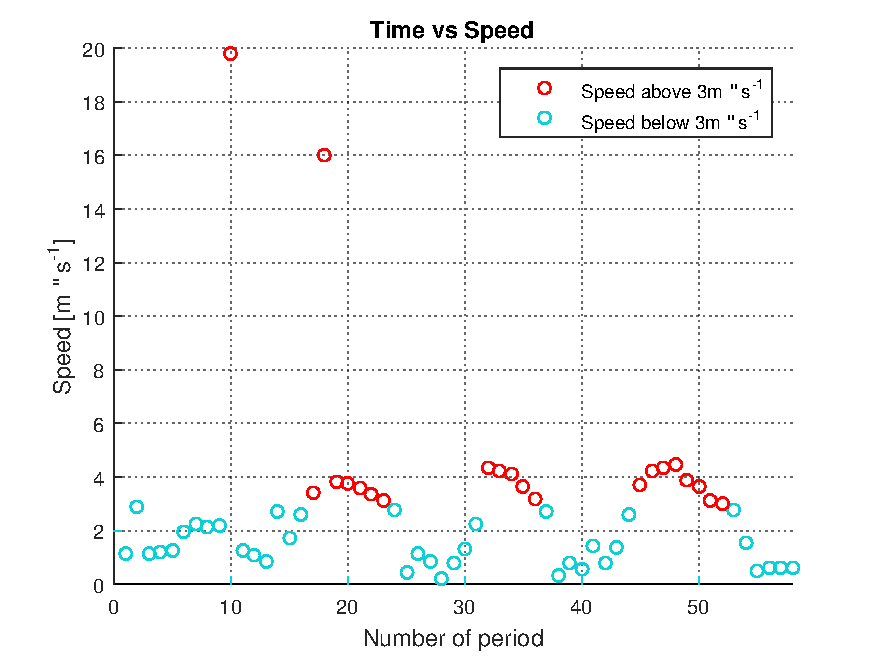
\includegraphics[scale=0.4]{Pictures/plot3.pdf}
\end{figure}

\end{frame}

%%%%%%%%%%%%%%% frame 4 %%%%%%%%%%%%%%%%%%%%


\begin{frame}{Acceptance Test}{Requirement 4}

\begin{table}[H] \centering
\begin{tabular}{|p{0.5cm}| p{7cm} |p{1cm}|}
\hline
\textbf{No.}  &  \textbf{Requirements} & \textbf{Done?}     \\ 
\hline
4 & The prototype must be able to access the route, which it has to follow, from a storage space located on the vehicle. & No \\ 
\hline
\end{tabular}
\end{table}
\end{frame}

%%%%%%%%%%%%%%%% frame 5 %%%%%%%%%%%%%%


\begin{frame}{Acceptance Test}{Requirement 5}

\begin{table}[H] \centering
\begin{tabular}{|p{0.5cm}| p{7cm} |p{1cm}|}
\hline
\textbf{No.}  &  \textbf{Requirements} & \textbf{Done?}     \\ 
\hline
5 & The prototype must be able to shut down, if the battery voltage is below its 
cut-off specification. & Yes \\ 
\hline
\end{tabular}
\end{table}
\end{frame}

%%%%%%%%%%%%%%%% frame 6 %%%%%%%%%%%%%%%%


\begin{frame}{Acceptance Test}{Requirement 6}

\begin{table}[H] \centering
\begin{tabular}{|p{0.5cm}| p{7cm} |p{1cm}|}
\hline
\textbf{No.}  &  \textbf{Requirements} & \textbf{Done?}     \\ 
\hline
6 & It shall be possible for the prototype to follow a predetermined route.  & No \\ \hline
\end{tabular}
\end{table}

  \pause

%%% Test 6 %%%
\begin{figure}[H]
  \centering
	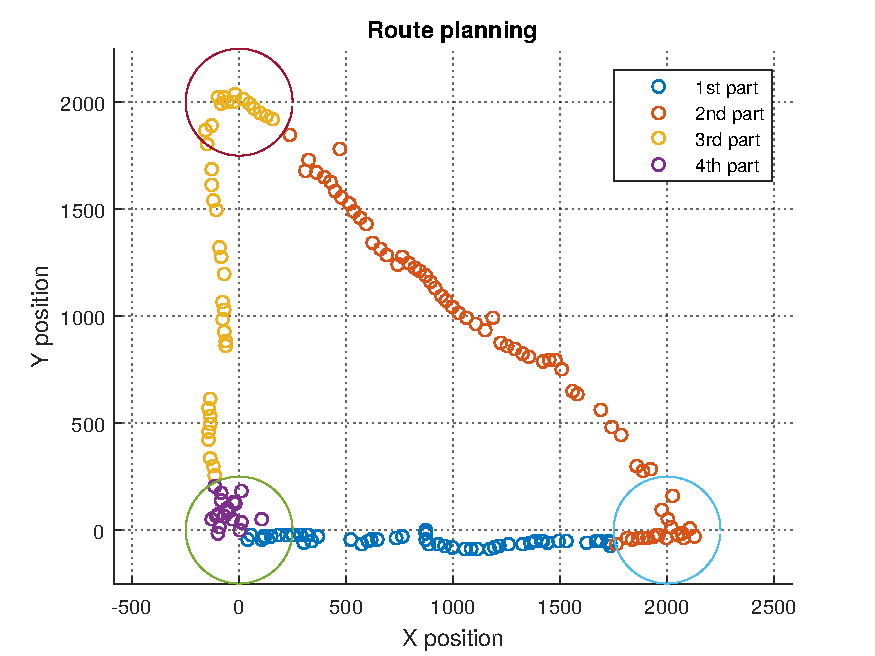
\includegraphics[scale=0.5]{Pictures/AccTest6.pdf}
\end{figure}
\end{frame}

%%%%%%%%%%%%%%%% frame 7 %%%%%%%%%%%%

\begin{frame}{Acceptance Test}{Requirement 7}

\begin{table}[H] \centering
\begin{tabular}{|p{0.5cm}| p{7cm} |p{1cm}|}
\hline%
\textbf{No.}  &  \textbf{Requirements} & \textbf{Done?}     \\ 
\hline%
7 & It shall be possible for the prototype to return to the predetermined route if disturbed.  & No \\ \hline
\end{tabular}
\end{table}

  \pause

%%% Test 7 %%%
\begin{figure}[H]
  \centering
	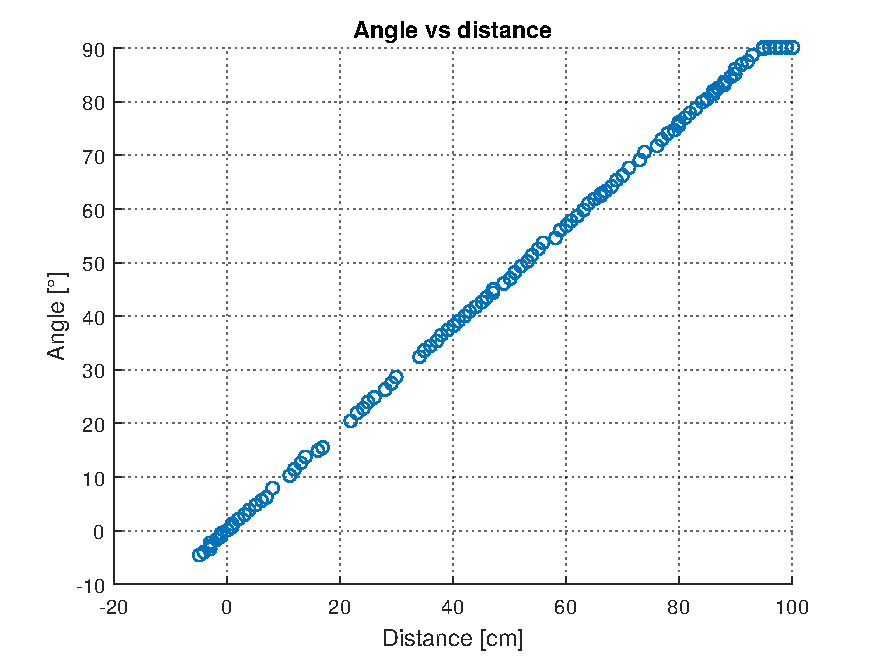
\includegraphics[scale=0.5]{Pictures/AccTest7.pdf}
\end{figure}


\end{frame}

%%%%%%%%%%%%%%%% frame 8 %%%%%%%%%%%%%%%


\begin{frame}{Acceptance Test}{Requirement 8}

\begin{table}[H] \centering
\begin{tabular}{|p{0.5cm}| p{7cm} |p{1cm}|}
\hline%
\textbf{No.}  &  \textbf{Requirements} & \textbf{Done?}     \\ 
\hline%
8 & The prototype shall be able to keep a velocity on 1,4 $m \cdot s^{-1}$, when going up or downhill and when turning.  & Yes \\ \hline
\end{tabular}
\end{table}

  \pause


  \begin{minipage}{\linewidth}
  	\begin{minipage}{0.45\linewidth}
  		\begin{figure}[H]
  			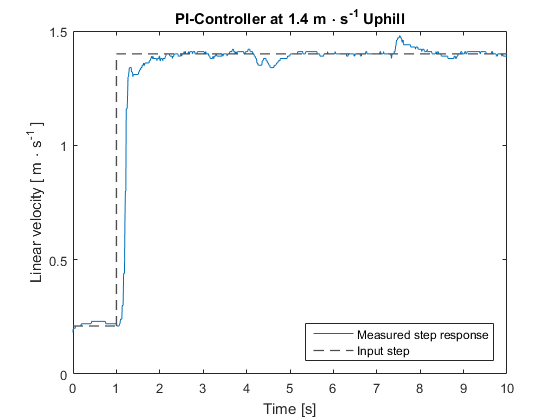
\includegraphics[scale=0.38]{Pictures/AccTest8U.png}
  			\centering
  			%\vspace{-.4cm}
  		\end{figure}
  	\end{minipage}
  	\hspace{0.03\linewidth}
  	\begin{minipage}{0.45\linewidth}
  		\begin{figure}[H]
  			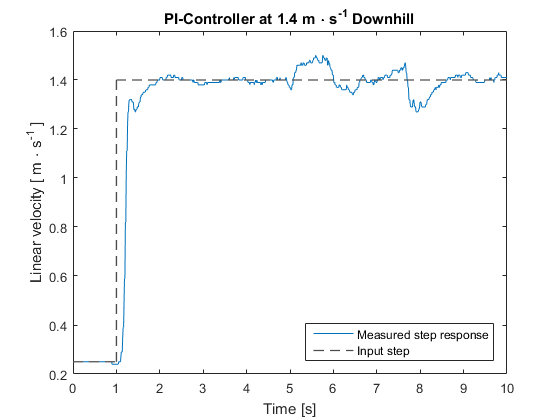
\includegraphics[scale=.38]{Pictures/AccTest8D.png}
  			\centering
  			%\vspace{-.4cm}
  		\end{figure}
  	\end{minipage}
  \end{minipage}

\end{frame}

%%%%%%%%%%%%%%%% END ACCEPTANCE TEST %%%%%%%%%%%%%%%



%%%%%%%%%%%%%%%%BEGIN CONCLUSION %%%%%%%%%%%%%%%
\subsection{Conclusion}

\begin{frame}{Conclusion}{What has been done?}

\pause

  \begin{itemize}
    \item<1-> Alternative navigation approaches with Games on Track system
    \item<2-> Belt vehicle analized to build prototype requirements
    \item<3-> Real Time Operating System implemented on the Arduino Mega
    \item<4-> XBee modules with protocol error handling
    \item<5-> Digital filter to lower the noise
    \item<6-> SD card storage
    \item<7-> Mathematical models simulated
    \item<8-> Distance model tests
    \item<9-> P and PI Controllers tested
  \end{itemize}
\end{frame}

%%%%%%%%%%%%%%%%END CONCLUSION %%%%%%%%%%%%%%%



%%%%%%%%%%%%%%%% BEGIN DISCUSSION %%%%%%%%%%
\subsection{Discussion}

\begin{frame}{Discussion}{What next?}

\pause

  \begin{block}{Functionalities missing from the requirements}
  	  The  steering controller could not be tested, because of magnetometer indoor disturbances.\\
      The non-volatile storage could be solved with more time.
  \end{block}
  
  \pause
  
  \textbf{What could we improve on this project?}
   \begin{itemize}
    \item<1-> The belt vehicle, not enough control
    \pause
    \item<2-> The GoT system, good accuracy but not large range
    \item<3-> Route planning and initial mapping
    \item<4-> Blade control
    \item<5-> Other functionalities (humidity, obstacle, or length detection) 
    \end{itemize}
\end{frame}
%%%%%%%%%%%%%%%% END DISCUSSION %%%%%%%%%%%%%






